\chapterimage{ChapterImages/Planning2}
\chapter{Planning}
\label{project-planning}

% %%%%%%%%%%%%%%%%%%%
% \begin{remark}\color{blue}
% Teams with global partners face special challenges in  terms of organization, project management and planning.
% It is a truism that organizational burden goes as the square of team size. 

% To address these issues, we ask each local+global team to prepare a \textbf{plan for Winter quarter} to include in this section. You have just accomplished a first, rough critical function prototype (CFP or CEP) and you have given a presentation and written a document that captures the current state of your vision and findings. You have learned who can do what and how much work it really takes. You are motivated to make Winter go more smoothly and to ``take control'' of your project instead of living from week to week.
% \normalcolor \end{remark}
% %%%%%%%%%%%%%%%%%%%

\vspace{1em}

In the following chapter we will evaluate what we did in the winter quarter, how we did it, which tools we used and which resources we allocated. Furthermore it contains an outlook into the spring quarter, our next steps and our personal reflections on the ME310-course at this point.

\section{Project Progress}

\subsection{Review of Winter Quarter}

During the fall quarter, we have explored different spaces between home and car, and successfully built a critical functional prototype (automatic car washing robot in the garage) as well as a critical experience prototype (a voice assistant inside the car to manage the home). At the end of the fall quarter, we arrived at a consensus that by talking about uniting home and car, we are focusing on smoothing the transition between those two places.

Therefore, during the winter quarter, both Stanford and HPI team built prototypes aiming to improve the not yet smooth experience when transiting between home and car. The Stanford team mainly focused on interaction within the home while HPI mainly focused on car related interaction before we eventually converged to car-home-transition related interaction for our last prototypes (also cf. figure \ref{fig:prototype_overview}). 

The Stanford team started with a critical function prototype, focusing on the leaving home experience. We designed a leave-home button that will prompt the user information about navigation, weather, things to bring and so on, preparing the coming trip for the user. The main takeaway was people might not want to have a nagging mom when leaving home and showing all the information through voice was not plausible. Then, in the dark horse prototype, instead of bringing the car to the home, we bring the home to the car, using the car as an extended room of the home. We built a movie theater and a sunshine meditation room in an SUV and it was actually much more plausible than we had thought before. For both the funky and functional system prototype, we built a physical device that sits inside home, showing information and sending a command upon leaving or arriving home. We designed a key fob storage unit that the user could set the scene of his home with by dropping the key fob into a certain beam that represented a lighting and audio scene. Then we realized that there was not a compelling enough use case that users would buy the device for. For the functional prototype, we decided to focus on security. We built a key fob storage case and with a screen that shows home and car status represented by different colors. Furthermore, it reduced false alarms because you could disarm your security system by dropping the key fob when you arrive home instead of entering a complex code.

The HPI team prototyped an in-car voice assistant during the fall quarter with which the smart home could be configured and controlled while in the car and driving, thus making use of otherwise wasted time in the car. The general feedback to it was positive, however for our dark horse prototype we went into a completely different direction to explore other possible orientations for the project. As suggested by the dark horse prototype, we went crazy and assumed teleportation is possible. We designed a shelf that can be placed anywhere inside the house and its compartments correspond to different compartments of the car such as the trunk or glove box. Whatever is placed in a compartment - whether it is in the shelf or the car - is automatically teleported to the corresponding other compartment as well, thus making carrying things from the car to the house unnecessary and enabling the user to pack things into the car without leaving the house. We found out that users especially liked that they do not have to carry their errands inside after doing the grocery shopping, and that they think they would forget less things if they had such a shelf serving as a kind of reminder since it is placed inside their apartment and they would have an overview over everything that is packed already. Based on the pain of having to carry groceries, we designed a self-driving cart that integrates seamlessly into the car as our funky prototype. We found out that people generally liked the idea of it, however we decided to go back to the reminder-need for our functional system prototype to better meet the constraints of our problem and the challenge as well as to converge with the Stanford team. As a result we came up with the AudiBits that can be placed anywhere inside the home and help the user to remember to pack things and to remember and check information about their car and home status.  

\begin{figure}
\centering
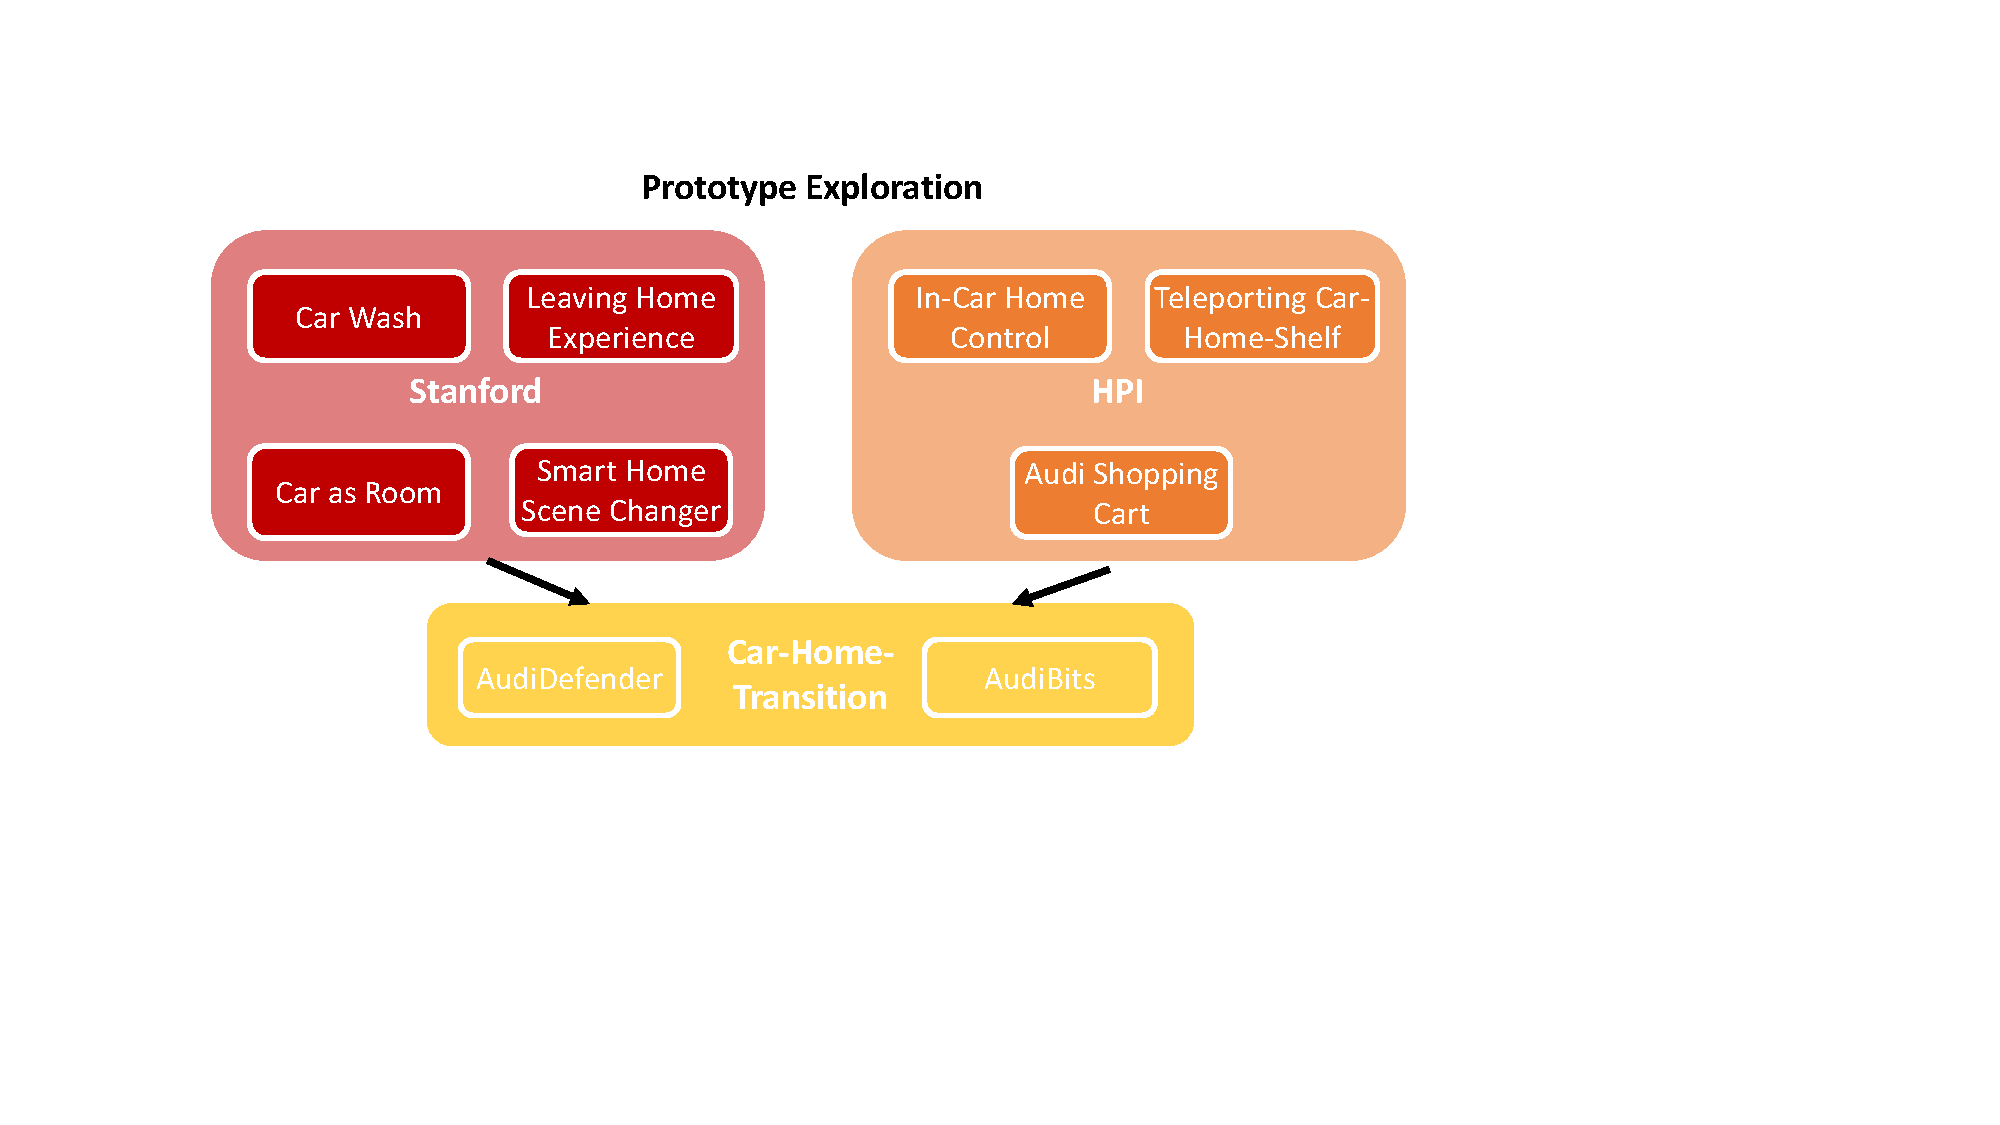
\includegraphics[width=5in]{Figures/Planning/Prototype_Overview}
	\caption{Overview over the prototypes created by Stanford and HPI during the fall and winter quarter.}
		\label{fig:prototype_overview}
\end{figure}

The Stanford team will visit the HPI from March 20th to March 27th. We are going to plan for the spring quarter and converge for the final design.

\subsection{Plan for Spring Quarter}
% Layout a plan for spring. Make sure your team reaches consensus on this. It is a critical element of how your liaisons (and the TTeam) will evaluate the status of your project. We will revisit this plan in spring SGMs.

%    What will your team do next? When \& how will milestones be accomplished, and by whom?
%    How will the budget be spent?
%    Any lessons learned from your time management this quarter?
%    How will you meet the final deadline of EXPE? 
The global team of students from HPI and Stanford will have its next in-person meeting the week after handing in this documentation. We will use this opportunity to fully converge our different approaches to the transition between home and car, in terms of visual design, the needs on which we base our design and the problem which we both are trying to solve. During this time we will also agree on which parts of the system which part of the team will implement (that is, if it is possible to split the system): With regards to the past prototypes and the background of the team members we can already determine that Stanford students have a penchant for good design and that HPI students are more focused on basing their implementations on needs discovered with their users so it would make sense to distribute tasks accordingly.

During the Spring Quarter we will keep our two weekly meetings to synchronize our activities as closely as possible given the time difference of 9 hours between HPI and Stanford students.

HPI students and Stanford students will meet again in Stanford at May 22nd to prepare for the final deadline. HPI students are willing to work full-time for the project to reach the final deadline.

\section{Team Management}
Each team decided to assign one team member to a certain area of responsibility (called "officer") to keep a better overview and split the workload. For HPI these were a space officer (Jonathan), a communication officer (Jonas), a financial officer (Johanna) and a documentation officer (Martin). Stanford had assigned roles of communication officer (Dylan), documentation officer (Maggie), and financial officer (Zhipeng) continuing from the fall quarter. Apart from introducing these roles on HPI side, we  did not make significant changes to our team management. 

\subsection{Communication and Collaboration}
We kept our timeslot of Friday, 10:00 AM PST and 7:00 PM CEST, for our weekly video conference. In addition to that, we held a second regular weekly meeting on Wednesday, 9:00 AM PST and 6:00 PM CEST, that we conducted in text chat form. This proved to be helpful, since it turned out to be a quite effective communication method with a built-in protocol.

We found that our agenda setting and strict moderation did not provide much added value last quarter. This could be due to the fact that we did not have good mechanisms in-place to review protocols of past meetings and follow up on action items. Our meetings in the winter quarter appeared to be less structured, but we did not notice a drop in the quality of our discussions.

\subsection{Used Tools}
For our video conferences we sticked to GoToMeeting. For the second weekly meeting in text form we used Slack. Regarding our documentation, we had discovered during the writing of our fall report that Overleaf had become very slow compiling our Latex files, so we re-evaluated our choice. We discovered that ShareLatex did the same job much quicker and are therefore using it now to collaboratively write this report.

We sticked to OneNote as our place to gather most of our documents and information. Over time, all team members started appreciating it as a valuable tool. During the winter quarter, we made it accessible for our liaisons for their reference. Complementing OneNote, we use OneDrive for the sharing of larger files - mainly photos and videos of testings and prototypes.
 
\section{Budget}
\label{sec:budget}

Both the HPI and the Stanford team are provided with a budget for buying necessary materials to conduct user studies and to build prototypes. The Stanford team has a dedicated budget for each quarter and unused budget rolls over to the next quarter. The HPI team has an overall budget for all three quarters.

\subsection{HPI Budget}

The HPI team has an overall budget of \euro5,500. At the current point the team has spent \euro320.88 for building prototypes and rewarding testers. A detailed list of the expenses of the current and the last quarter can be found in table \ref{tab:budget_hpi}. The HPI team has only spent a very small fraction of its budget so far since no electronics and only very basic prototyping materials were needed. We expect to spend more money in the coming quarter when it comes to implementing and realizing technical solutions but we believe that we will not have any problems staying within the remaining budget. 

\begin{table}[!ht]
	\centering
		\begin{tabular}{| r | r | r |}
		%\begin{tabular}{| p{50mm} | p{17mm} | p{17mm} |}
		\hline
		\textbf{Purpose}	& \textbf{Date} & \textbf{Amount} \\
		\hline
		Chocolate for participants of user study & 11/23/2015 & \euro21.18\\ \hline
        \multicolumn{2}{|r}{\textbf{Spending Fall Quarter:}} & \textbf{\euro21.18} \\ \hline
        Chocolate for participants of user study & 01/23/2016 & \euro29.70 \\ \hline
        Equipment for Dark Horse testing (shelf and things to pack) & 01/27/2016 & \euro47.78 \\ \hline
        Preparation of Dark Horse testing car & 01/27/2016 & \euro35.89 \\ \hline
        Material for Funky Prototype (hand truck, tape, boxes) & 02/03/2016 & \euro94.67 \\ \hline
        Shopping vouchers for Funky-testers & 02/06/2016 & \euro75.00 \\ \hline
        Collaborative LaTeX license (ShareLaTeX) & 03/14/2016 & \euro16.66 \\ \hline
        \multicolumn{2}{|r}{\textbf{Spending Winter Quarter:}} & \textbf{\euro299.70} \\ \hline \hline
        \multicolumn{2}{|r}{\textbf{Spending Total:}} & \textbf{\euro320.88} \\ \hline
        \multicolumn{2}{|r}{\textbf{Remaining Budget:}} & \textbf{\euro5,179.12} \\ \hline
	\end{tabular}
	\caption{HPI Budget Overview }
	\label{tab:budget_hpi}
\end{table}
    
\subsection{Stanford Budget}

The Stanford team has an annual budget of \$8000, and overall we have spent only a small fraction of it during the fall and winter quarter. Most the spending is related to benchmarking hardware, prototyping electronics, German Visa, and the SUDS. Considering the anticipatory spending for fall and winter, we have plenty of them left for Spring quarter. 

Given that our prototype will focus on the physical interface of car and home, and due to simplicity issue, we will simulate most of the information flow and activities at the car side and home side. And for spring quarter, most of the spending would be related to prototyping electronics and manufacturing parts. Since we may explore other interfaces, such as gesture control and hologram, the cost associated with these novel hardware would be much higher. Overall, according to the speed of current spending, we believe we have enough budget for spring development, and it is highly possible that we have some budget left at the end of the year.   

\begin{table}[!ht]
	\centering
		\begin{tabular}{| r | r | r |}
		%\begin{tabular}{| p{50mm} | p{17mm} | p{17mm} |}
		\hline
		\textbf{Purpose}	& \textbf{Date} & \textbf{Amount} \\
		\hline
		Benchmarking smart home hardwar & 11/2/2015 & \$150.01 \\ \hline
		Benchmarking at Target Open House & 11/1/2015 & \$44.16 \\ \hline
		CFP, car body pieces  & 11/15/2015 & \$14.31 \\ \hline
		CFP, cloth, towel, cleaning solution etc.  & 11/14/2015 & \$46.83 \\ \hline
		Fall Team Mileage   & 12/1/2015 & \$64.41 \\ \hline
		Working meal with liasons  & 12/6/2015 & \$117.10 \\ \hline
        \multicolumn{2}{|r}{\textbf{Spending Fall Quarter:}} & \textbf{\$436.82} \\ \hline
        CEP, car rental & 1/19/2016 & \$62.48 \\ \hline	
        Darkhorse, lights for prototyping & 1/24/2016 & \$179.91 \\ \hline	
        Benchmarking gestural interface, and augmented reality & 1/31/2016 & \$141.69 \\ \hline
        Prototyping, 2 Raspberry Pi starter Kit & 2/2/2016 & \$139.98 \\ \hline	
        Electronics, RF transducers, speaker, pressure sensor, etc. & 2/3/2016 & \$78.07 \\ \hline	
        German Visa Related for Zhipeng and Maggie & 2/16/2016 & \$266.19 \\ \hline
        Prototyping, Wireless Outlets, Switch, LCD etc. & 2/6/2016 & \$76.10 \\ \hline	
        RFID modules, LEDS, sensors and accessories & 2/18/2016 & \$133.09 \\ \hline	
        Modeling Material & 2/21/2016 & \$39.09 \\ \hline
        PLX Bluetooth Module and Dongle & 2/5/2016 & \$72.30 \\ \hline
        Prototyping, Logic Analyzer & 2/11/2016 & \$126.85 \\ \hline
        Functional, Large Battery Bank & 2/23/2016 & \$40.90 \\ \hline
        SUDS & 2/10/2016 & \$476.20 \\ \hline
        Winter Team Mileage & 3/1/2016 & \$52.38 \\ \hline
        \multicolumn{2}{|r}{\textbf{Spending Winter Quarter:}} & \textbf{\$1,885.23} \\ \hline \hline
        \multicolumn{2}{|r}{\textbf{Spending Total:}} & \textbf{\$2,322.05} \\ \hline
        \multicolumn{2}{|r}{\textbf{Remaining Budget:}} & \textbf{\$5,677.95} \\ \hline
	\end{tabular}
	\caption{Stanford Budget Overview }
	\label{tab:budget_stanford}
\end{table}

\section{Reflections}
\subsection*{Martin Fritzsche}
I choose to take part in the ME310 course because of the prospect of gaining insights into a totally different approach on how to tackle a project and exercising this from the very beginning up to a pretty much presentable prototype. The design thinking process was completely new to me at the beginning of the course, which imposed quite some challenges. I sometimes felt a little lost and was very thankful to have my team partners which had some previous knowledge of the process and thus could guide and jump in by giving a more concise frame on what to do at which stage. Right now I have a pretty good idea of the process and feel like I am actively contributing.

That last three months passed by very quickly. While building and testing our different prototypes we explored more and more of the design space and found some interesting directions to follow. With the latest prototypes from Stanford and HPI imagined as two sides of the same system we finally have a unified vision down the road, something that I found hard to see before.

I like the structure of the course with the weekly presentations in a not-to-formal matter. They help by forcing us to rethink the week and put our findings in a nutshell. I am still amazed by our results week after week, since at the beginning of every week I mostly felt overwhelmed by all the possible directions to explore and tasks to fulfill. It felt hard to try to converge in one direction after having explored such a wide variety of ideas. 

Working together with our Stanford team partners has been working out very well. I very much look forward to the visit of our partner team next week. We planned an intensive week, discussions and planning on a unified vision and prototype to go for in our final three months 

I am confident that we can keep up our good spirit and build an intriguing and original prototype.
\subsection*{Jonathan Herdt}
\subsection*{Zhipeng Hu}
ME310 is a challenging and rewarding process. In this environment, I am able to adapt to some behavior pattern of design communities, which is refreshing and complementary to my engineering mind. More specifically, in this quarter, I improved communication skills and learned empathy in decision process. A major part about winter quarter is how to embrace uncertainty, it is definitely more challenging than it firstly sounds to me. It requires remarkable self-motivation for every team member. I appreciate very much the unique contribution of my team, we are always able to make things happen. 

A consensus among Stanford team is that we should do a better job at selling a vision and product. For some of the SGMs, we could make it better by articulating a story that emphasize one aspect of the problem or need. And the effect also depends on the way we present it, more enthusiasm is important. Moreover, I wish we could do a better job at persona and needfinding, it seems we need a model that did a good job at this to guide us. From one of the other teams, I heard we should have persona first to perform needfinding and interviews. Not to say that we should have that fixed paradigm, but determining persona first may help us have a priority of demographic that will leads to more meaningful needfinding. 

During this design process, I become realized that it is really an art to stay united as a team and make every team member inspired. We will aim at the goal to have a team performance greater than the sum of the individual. And I feel, that is those subtle empathy, understanding and enthusiasm that makes this happen.

\subsection*{Jonas Kemper}
The fall and winter quarter of ME310 appeared very differently to me. Where the fall quarter felt like a series of sprints, the winter quarter felt more like a marathon. This could be due to the fact, that we had very tight deadlines for the CEP and CFP prototypes. In the winter quarter we had longer timeslots for each prototype so we could plan longterm and try out different strategies for time management.

What I really like about ME310 is that it feels much more like a real world project than most other university courses. There are many parties involved in every project and individuals have diverse cultural backgrounds. Moreover, the motivation and goals of the different parties do not always align perfectly. This makes it a uniquely interesting challenge to carefully balance the different interests. Keeping an effective process going and constantly trying to improve it is an on-going learning journey and has been taking us non-negligible amounts of time --- which is a good thing, I think.

Regarding the design process itself, I occasionally find myself wondering, whether most design projects feel like this or if there is something unique about our particular challenge. Sometimes I feel like the constraints of our challenge are pretty narrow and wide open at the same time. This can make it hard to see a clear direction that we are moving along. But then again, as always in life, many things start only to make sense in retrospect.

\subsection*{Johanna Latt}
\subsection*{Dylan Moore}
ME 310 continues to be a challenge and an amazing experience. I've been amazed how different my mindset has been the past few weeks as opposed to Fall Quarter. Moving from the divergent "let's try anything" phase to the convergent "we actually need to build something that works" phase has been a challenge. But absolutely good practice and it has been very informative. I find it hard to articulate what explicit "skills" that I've gained up to this point, only knowing for sure that I have implicitly gained more experience as a designer, and believe that it's that implicit knowledge and experience that is most useful moving forward. As Barry Katz said in a lecture at Stanford recently, "design thinking" is nothing but the accumulated experience of a century's worth of design practice. 

Our project ended up being quite more challenging than I anticipated - we expected the smart home as it is and will be to fulfill more compelling user needs than it does. From our benchmarking and needfinding, we found the smart home is more about convenience innovation than addressing latent user needs. As a result, working within that space has been more frustrating than exciting at times. However, the vision that we have as a unified team now is interesting, does address a compelling need, even if it may be at the fringes of what we considered the "smart home" back in October, and I believe that we can make the implementation spectacular and really design a system that wows users at EXPE. We have had a rather generic persona up to this point, as we find the needs we are addressing widely applicable, but perhaps by narrowing that down, we can enhance our implementation. There is also much to be said for the explicit experience and interaction that we will design.

I am pleasantly surprised how close the HPI and Stanford developments ended up at the end of the quarter, and that bodes well for our unified vision going forward. We have worked very well as a team, staying productive, professional, and empathetic, even when things got frustrating or busy, and I am very much looking forward to all of us getting together in Berlin for Spring Break. I believe all of our work leading up to this point has prepared us well for the experiences to come in Spring Quarter.


\subsection*{Maggie Xu}
Winter quarter turned out to be much more challenging and rewarding than I'd thought before. Compared to fall quarter when we mostly focused on brainstorming and exploring, this quarter we have got our hands dirty in continuous prototype challenges. I really appreciate our efforts as a team to deliver satisfying functional prototypes as well as to overcome the difficulty when we literally had no idea about future steps. 

Throughout the prototyping process, I had a better understanding of learning by doing. I took an Android programming class this quarter, but it was until we had to design an Android interface which communicated with RPi through bluetooth in ME310 that I started to appreciate android app development process. 

I'm glad that Stanford and HPI gradually converged after separately exploring various areas for the past two quarters. International communication is a challenge and it's really helpful that we decided to have another message meeting besides our regular weekly video meeting. I'm looking forward to meeting HPI teammates in Berlin this spring break, and I believe we will have a better sense of what we are going to implement in spring quarter afterwards.

